
\begin{frame}
	$q(x_{t-1} | x_t, x_0) = \mathcal{N}\left(x_{t-1} ; \tilde{\mu}_{t}(x_t, x_0), \tilde{\beta}_t I\right)$
	$q(x_{t-1} | x_t, x_0) = \mathcal{N}\left(x_{t-1} ; \tilde{\mu}_{t}(x_t, x_0), \tilde{\beta}_t I\right)$
	
	$\tilde{\mu}_{t}(x_t, x_0) = \frac{\sqrt{\bar{\alpha}_{t-1}} (1 - \alpha_t)}{1 - \bar{\alpha}_t} x_0 + \frac{\sqrt{\alpha_t} (1 - \bar{\alpha}_{t-1})}{1 - \bar{\alpha}_t} x_t$
	$\tilde{\mu}_{t}(x_t, x_0) = \frac{\sqrt{\bar{\alpha}_{t-1}} \beta_t}{1 - \bar{\alpha}_t} x_0 + \frac{\sqrt{\alpha_t} (1 - \bar{\alpha}_{t-1})}{1 - \bar{\alpha}_t} x_t$
	
	$\tilde{\beta}_t = \frac{1 - \bar{\alpha}_{t-1}}{1 - \bar{\alpha}_t} \beta_t$
	$\tilde{\beta}_t = \frac{1 - \bar{\alpha}_{t-1}}{1 - \bar{\alpha}_t} (1 - \alpha_t)$
	
\end{frame}





\begin{frame}{Forward Diffusion Process}
%	 & \text{ ;where } \boldsymbol{\epsilon}_{t-1}, \boldsymbol{\epsilon}_{t-2}, \dots \sim \mathcal{N}(\mathbf{0}, \mathbf{I})
\small
\begin{itemize}[]
	\item Đặt $\alpha_t = 1 - \beta_t$, $\bar{\alpha}_t = \prod_{i=1}^t \alpha_i$
\end{itemize}
\vspace{-15pt}
\begin{align*}
	\mathbf{x}_t & = \sqrt{\alpha_t}\mathbf{x}_{t-1} + \sqrt{1 - \alpha_t} \boldsymbol{\epsilon}_{t-1} \\
						& = \sqrt{\alpha_t \alpha_{t-1}} \mathbf{x}_{t-2} + \sqrt{1 - \alpha_t \alpha_{t-1}} \bar{\boldsymbol{\epsilon}}_{t-2} \\
						& = \dots \\
						& = \sqrt{\bar{\alpha}_t}\mathbf{x}_0 + \sqrt{1 - \bar{\alpha}_t}\boldsymbol{\epsilon} \\
						q(\mathbf{x}_t \vert \mathbf{x}_{t-1}) &= \mathcal{N}(\mathbf{x}_t; \sqrt{\alpha_t} \mathbf{x}_{t-1}, (1 - \alpha_t)\mathbf{I}) \\ 
						\rightarrow q(\mathbf{x}_t \vert \mathbf{x}_0) &= \mathcal{N}(\mathbf{x}_t; \sqrt{\bar{\alpha}_t} \mathbf{x}_0, (1 - \bar{\alpha}_t)\mathbf{I})
\end{align*}
\vspace{-20pt}
%\begin{figure*}
	
%	& \text{ ;where } \bar{\boldsymbol{\epsilon}}_{t-2} \text{ merges two Gaussians (*).} \\
\begin{columns}
\begin{column}{0.5\textwidth}
	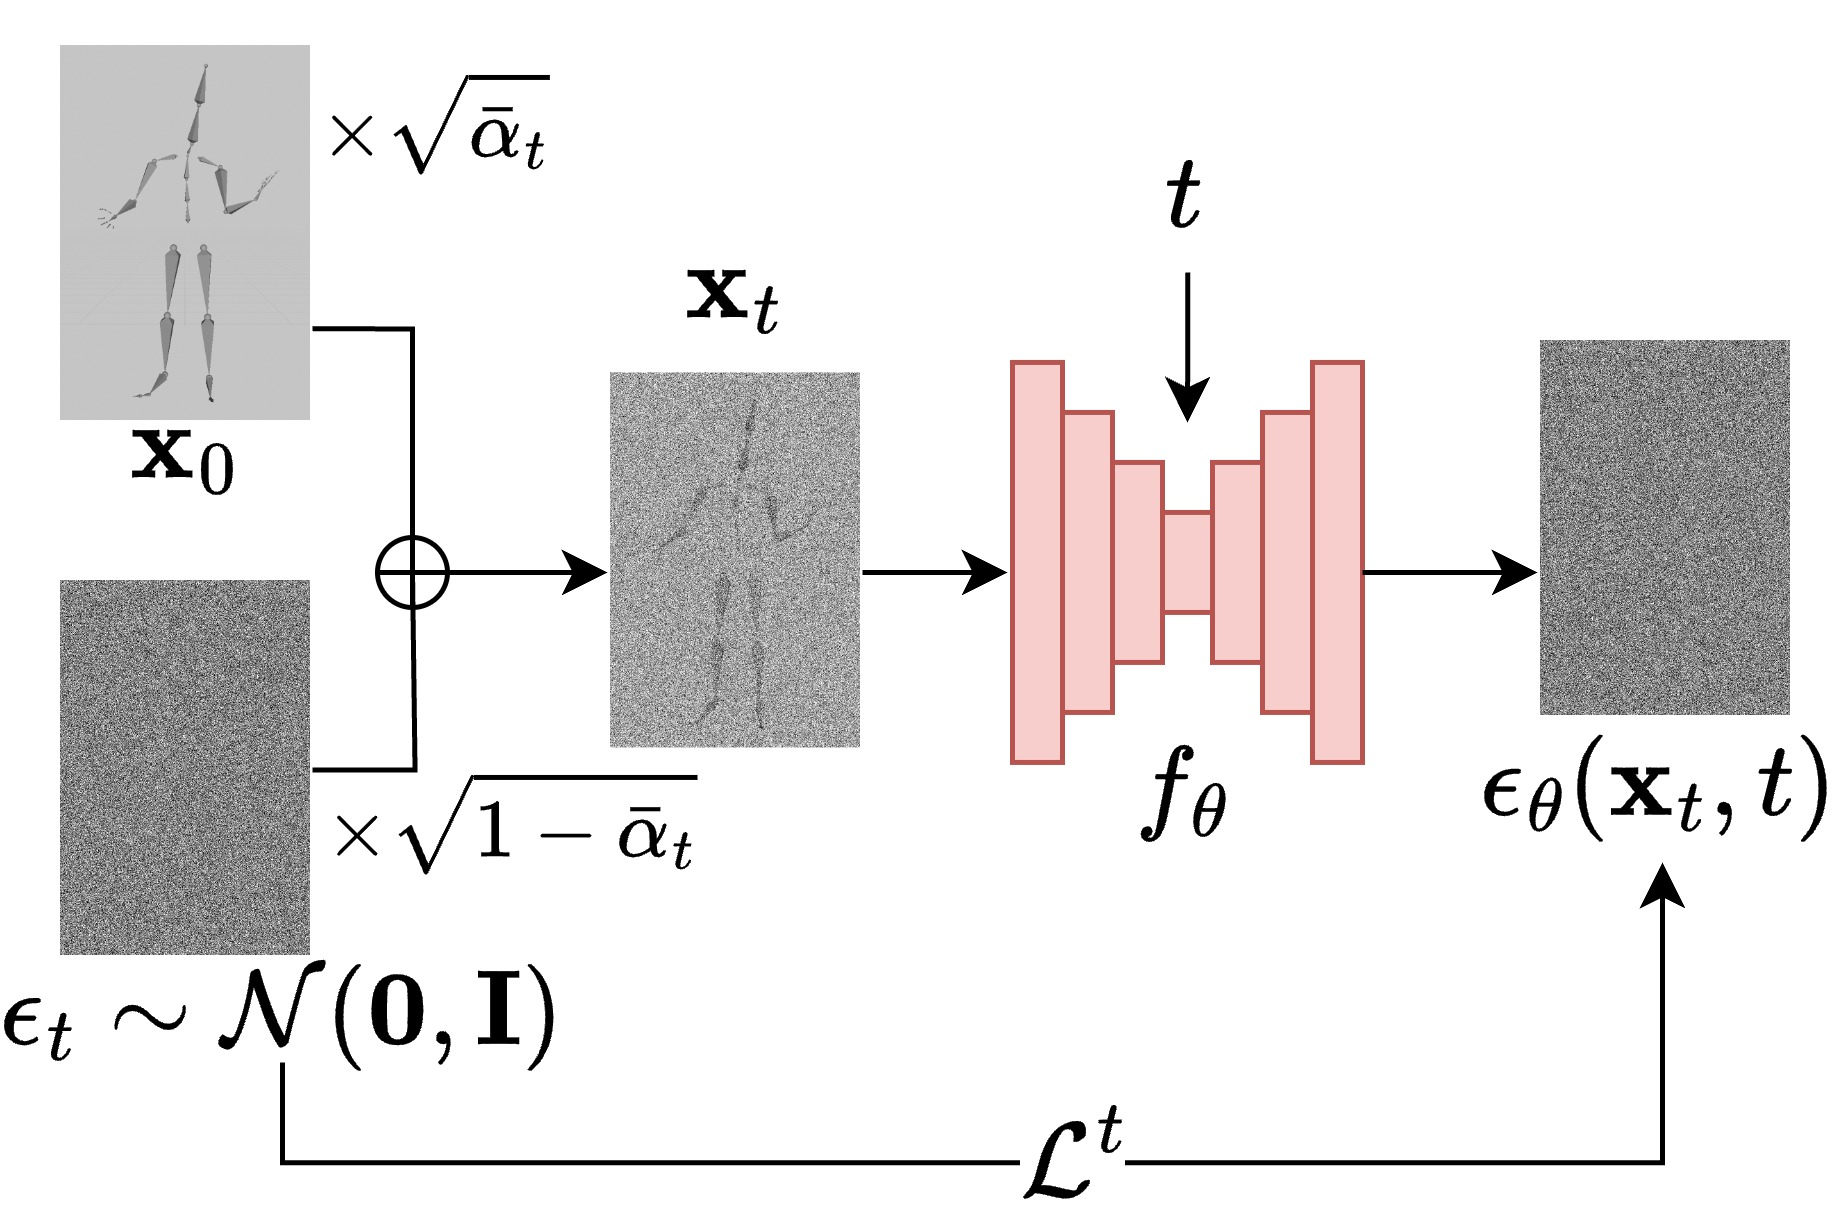
\includegraphics[width=\textwidth]{AlgorithmForwardDiffusion.png}
\end{column}


	
\begin{column}{0.5\textwidth}
	\footnotesize
	\begin{algorithm}[H]
		\caption{Training} \label{alg:training}
		\begin{algorithmic}[1]
			\footnotesize
			\Repeat
			\State $\bx_0 \sim q(\bx_0)$
			\State $t \sim \mathrm{Uniform}(\{1, \dotsc, T\})$
			\State $\bepsilon\sim\mathcal{N}(\bzero,\bI)$
			\State Take gradient descent step on
			\Statex $\qquad \grad_\theta \left\| \bepsilon - \bepsilon_\theta(\mathbf{x}_t, t) \right\|^2$
			\Until{converged}
		\end{algorithmic}
	\end{algorithm}
\end{column}
\end{columns}
\end{frame}

\begin{frame}{Reverse Diffusion Process}
	
\small
$p_{\theta}(\mathbf{x}_T) = \mathcal{N} (0, \mathbf{I}) \qquad 
p_{\theta}(\mathbf{x}_{t-1} | \mathbf{x}_t) = \mathcal{N}(\mathbf{x}_t; \mu_\theta(\mathbf{x}_t), \sigma_t^2 \mathbf{z})
$
%\begin{columns}
%	\begin{column}{0.5\textwidth}
%		
%	\end{column}
%	\begin{column}{0.5\textwidth}
%		
%	\end{column}
%\end{columns}

$\mu_\theta(\mathbf{x}_t) = 
\frac{1}{\sqrt{\alpha_{t}}} ( \mathbf{x}_t - 
\frac{1-\alpha_t}{ \sqrt{1 - \bar{\alpha_{t}} }}
\epsilon_{\theta} (\mathbf{x}_t,t))$
%\vspace{-20pt}
%\begin{figure*}

%	& \text{ ;where } \bar{\boldsymbol{\epsilon}}_{t-2} \text{ merges two Gaussians (*).} 

\begin{columns}
	\begin{column}{0.43\textwidth}
		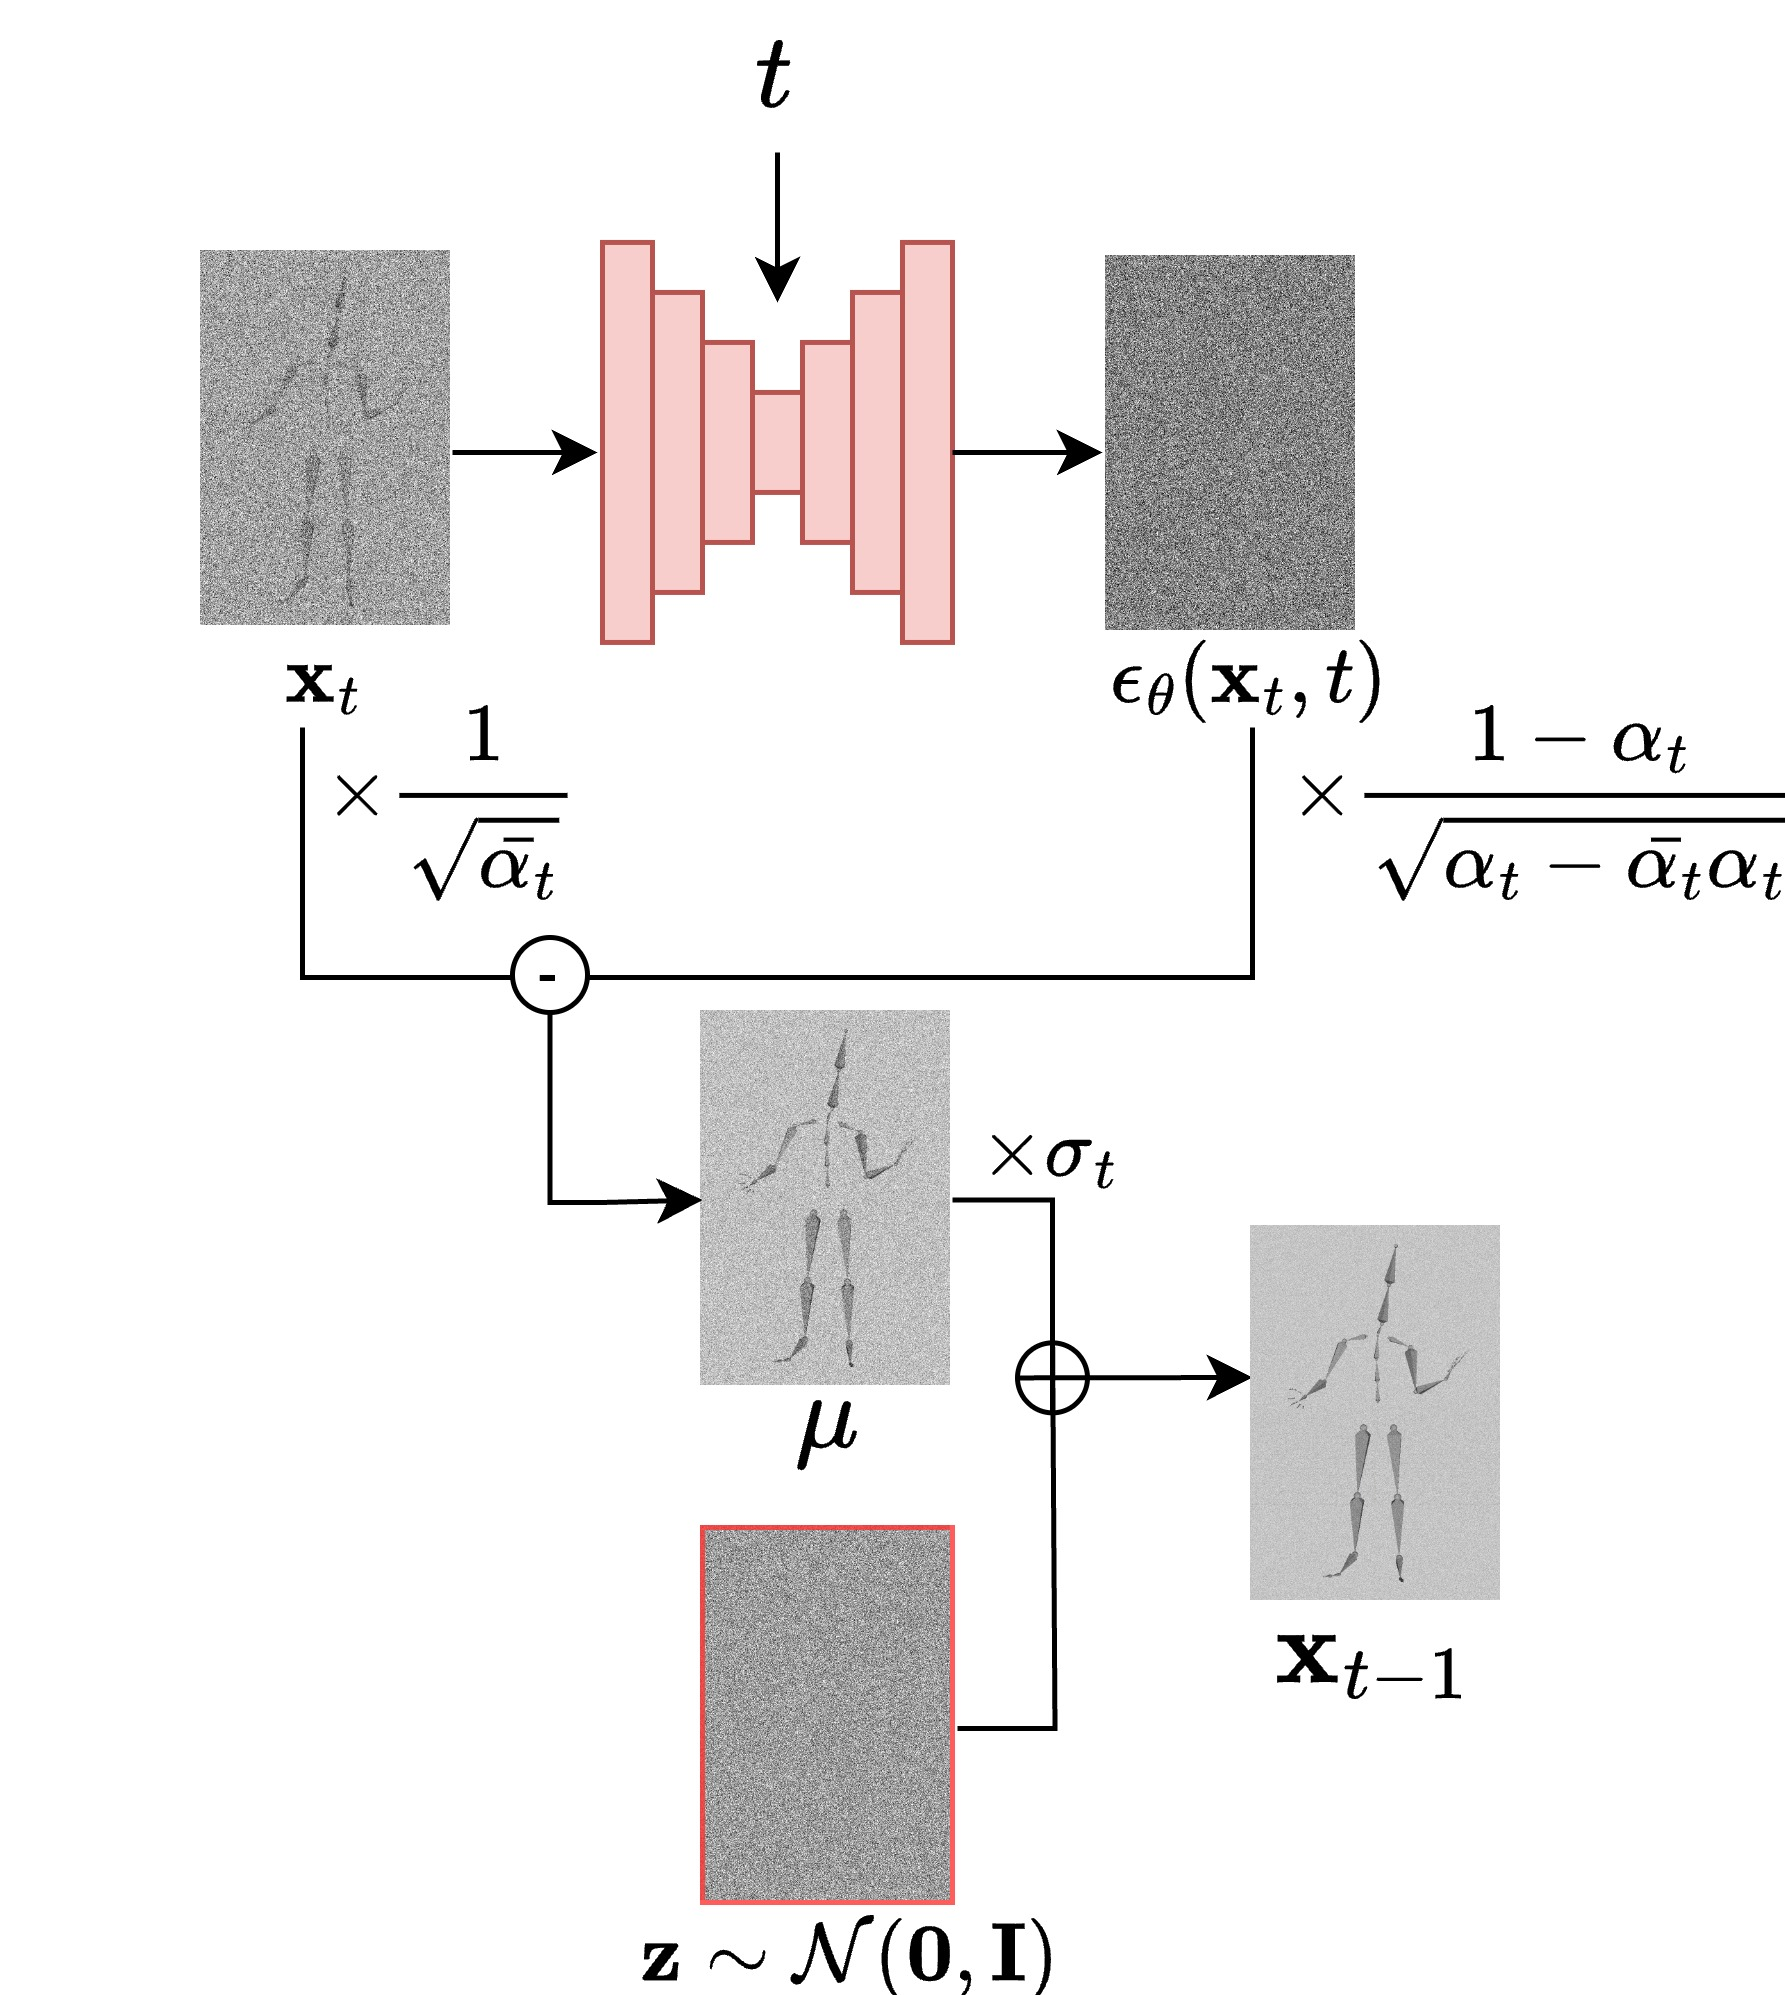
\includegraphics[width=\textwidth]{AlgorithmSamplingDiffusion.png}
	\end{column}
	
	\begin{column}{0.57\textwidth}
		\footnotesize
		\begin{algorithm}[H]
			\caption{Sampling} \label{alg:sampling}
			\footnotesize
			\begin{algorithmic}[1]
					\footnotesize
					\State $\bx_T \sim \mathcal{N}(\bzero, \bI)$
					\For{$t=T, \dotsc, 1$}
					\State $\bz \sim \mathcal{N}(\bzero, \bI)$ if $t > 1$, else $\bz = \bzero$
					\State $\mu = \frac{1}{\sqrt{\alpha_t}}\left( \bx_t - \frac{1-\alpha_t}{\sqrt{1-\bar\alpha_t}} \bepsilon_\theta(\bx_t, t) \right) $
					\State $\bx_{t-1} = \mu + \sigma_t \bz$
%					+ \sigma_t \bz
%_\theta (\mathbf{x}_t,	 t)
					\EndFor
					\State \textbf{return} $\bx_0$
					\vspace{.04in}
				\end{algorithmic}
		\end{algorithm}
\end{column}

\end{columns}

\end{frame}

%	\algrenewcommand\algorithmicindent{0.5em}
%	\begin{figure}[t]
	%		\begin{minipage}[t]{0.495\textwidth}
		%			\begin{algorithm}[H]
			%				\caption{Training} \label{alg:training}
			%				\small
			%				\begin{algorithmic}[1]
				%					\Repeat
				%					\State $\bx_0 \sim q(\bx_0)$
				%					\State $t \sim \mathrm{Uniform}(\{1, \dotsc, T\})$
				%					\State $\bepsilon\sim\mathcal{N}(\bzero,\bI)$
				%					\State Take gradient descent step on
				%				\Statex $\qquad \grad_\theta \left\| \bepsilon - \bepsilon_\theta(\sqrt{\bar\alpha_t} \bx_0 + \sqrt{1-\bar\alpha_t}\bepsilon, t) \right\|^2$
				%					\Until{converged}
				%				\end{algorithmic}
			%			\end{algorithm}
		%		\end{minipage}
	%		\begin{minipage}[t]{0.495\textwidth}
		%			
		%		\end{minipage}
	%		\vspace{-1em}
	%	\end{figure}




	
%	
%		if $L$ is not known (usually the case), can use the following line search:
%	\noindent\rule[-5pt]{\textwidth}{0.4pt}
%	
%	\noindent\rule[10pt]{\textwidth}{0.4pt}
%	
%	typical value of $\beta$ is $1/2$, and 
%	\[
%	\hat{f}_\lambda(x,y) = f(y) + \nabla f(y)^T (x - y) + 
%	(1/2\lambda)\|x - y\|_2^2
%	\]